
% ------------------------------------------------------------------------------------------------------------------------------------------
% Direct solvers
% ------------------------------------------------------------------------------------------------------------------------------------------
\section{Direct Poisson solvers in FDS} 
\label{SEC_SCARC_direct_solvers}
At a first glance, the ongoing improvements in the current computer technology motivate the use of direct methods such as the Gaussian elimination method and its variants for symmetric, positive definite matrices for the solution of the elliptic equations. Another extremely powerful class of direct methods which is successfully used in many different branches of science is based on spectral solvers. 
Both classes will be explained in more detail below.

Direct solvers compute the solution of a system of equations within a possibly very complex step without intermediate approximations. They may be performed with enormous speed and are often used for the demonstration of potential computer power, see e.g.\ the LINPACK-tests by~\cite{Dongarra:1998}.
They have proven to be very robust even in the non-symmetric and ill-conditioned case. Besides, they are nearly independent of the  degree of grid distortion (except for rounding errors) and well suited for the application on unstructured grids.  
In contrast to iterative methods, they are completely independent of whether a good starting solution exists or not, but they also do not benefit if this is already the case. They achieve a high level of computational accuracy, but they do not benefit if this is not required at all.

However, as already mentioned, the development of corresponding parallel analogues is highly complicated.
Most often, reasonably efficient strategies follow purely algebraic considerations
and are not conforming with geometrically motivated domain decompositions strategies.
Nevertheless, for  moderately sized problems, especially if only one or a few sub-meshes are used, direct solvers are incomparably fast and should generally be preferred over iterative ones.
Typically, there is a critical number of subdomains for which the parallelization overhead dominates the numerical efficiency associated with the original serial methodology which should be analyzed carefully.
 
 

% ------------------------------------------------------------------------------------------------------------------------------------------
% FFT solver
% ------------------------------------------------------------------------------------------------------------------------------------------
\subsection{Parallel FFT with Pressure Iteration}
\label{SEC_SCARC_fft_solver}

Spectral solvers like the {\it Fast Fourier Transformation} (FFT) exploit a very special property of the underlying Poisson problem, namely that sine and cosine functions are eigenvectors of the Laplace operator. They expand the solution as a Fourier series which can be quickly performed at rather low complexity. In practice, this approach has proven to be highly efficient and is used in many different fields of application. However, FFT methods are restricted to structured grids which may impede the use for complex geometries.

As described in detail in the FDS Technical Guide~\cite{McGrattan:2018:TG}, the pressure equation (\ref{EQ_SCARC_pressure}) is obtained from the momentum equation by a sequence of substitutions and simplifications. The major advantage of this derivation is that it finally leads to a system of equations which has constant coefficients (i.e.\ is separable). 
Since FDS furthermore relies on the use of cubic meshes each with structured rectangular grids each, it is possible to use a highly optimized FFT solver from the CRAYFISHPAK~\cite{Sweet::Crayfishpak}.
%
In the single-mesh case only one globally acting FFT-method is performed which has proven to be extremely powerful and fast over the past years. 
In the multi-mesh case every sub-mesh performs its own local FFT in order to compute an exact solution to the related local Poisson problem as illustrated in Fig.~\ref{FIG_SCARC_local_ffts}. The global solution is then composed from the local ones.
\begin{figure}[ht]
\begin{center}
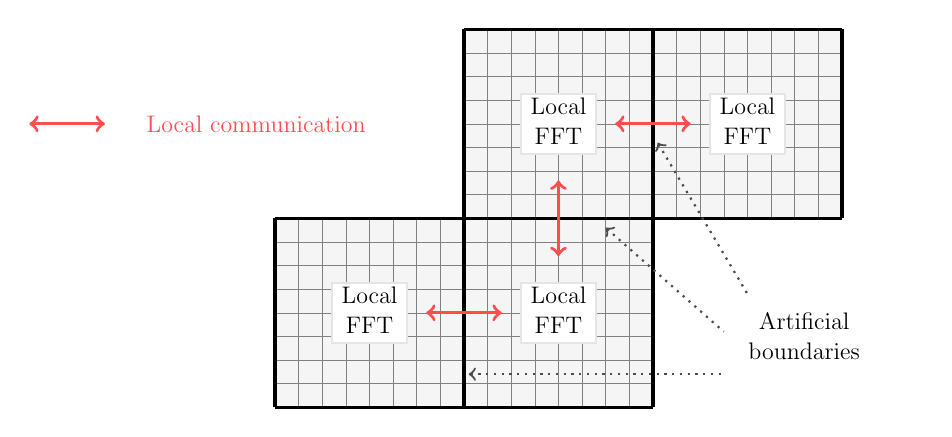
\begin{tikzpicture}
[
scale=0.6,
every node/.style={scale=0.6},
Background/.style={rectangle,draw=black!04,fill=black!04, thin, minimum size = 4 cm},
Obstruction/.style={rectangle,draw=black!70,fill=black!40, very thick, minimum size=1cm},
Finegrid/.style={step=0.5cm,gray,very thin},
Thickline/.style={-,draw=black!100,fill=black!02, very thick},
Thinline/.style={draw=black!100,fill=black!02, very thin},
Ball/.style={circle, draw=black!40, fill=red!20, thin, minimum size=3.5mm},
Circle/.style={circle,draw=black!40,fill=black!06,thin,minimum size=35.5mm},
Rectangle/.style={rectangle,draw=black!10,fill=white,inner xsep=0pt, inner ysep=0pt,},
Box/.style= {very thin, rectangle, inner xsep=10pt, inner ysep=10pt,},
ComArrow/.style= {<->,very thick, draw=red!70,},
DotArrow/.style= {<-, thick, dotted, draw=black!70,},
]

\node[Background] at (  2,2) {};
\node[Background] at (  6,2) {};
\node[Background] at (  6,6) {};
\node[Background] at (10,6) {};

\node[Obstruction] at (2,2) {};

\draw[Finegrid] (0,0) grid (  8,4);
\draw[Finegrid] (4,4) grid (12,8);

\draw[Thickline] (0,0)--(  8,0);
\draw[Thickline] (4,8)--(12,8);
\draw[Thickline] (0,4)--(  4,4);
\draw[Thickline] (8,4)--(12,4);

\draw[Thickline] (  0,0)--(  0,4);
\draw[Thickline] (  4,8)--(12,8);
\draw[Thickline] (  4,4)--(  4,8);
\draw[Thickline] (  8,0)--(  8,4);
\draw[Thickline] (12,4)--(12,8);

\draw[Thickline] (4,0)--(4,4);
\draw[Thickline] (4,4)--(8,4);
\draw[Thickline] (8,4)--(8,8);

\node[Rectangle] at (  2,2.0) {\Large \begin{tabular}{c} Local \\ FFT\end{tabular}};
\node[Rectangle] at (  6,2.0) {\Large \begin{tabular}{c} Local \\ FFT\end{tabular}};
\node[Rectangle] at (  6,6.0) {\Large \begin{tabular}{c} Local \\ FFT\end{tabular}};
\node[Rectangle] at (10,6.0) {\Large \begin{tabular}{c} Local \\ FFT\end{tabular}};

\draw[ComArrow](3.2,2)--(4.8,2);
\draw[ComArrow](6,3.2)--(6,4.8);
\draw[ComArrow](7.2,6)--(8.8,6);

\draw [DotArrow] (8.1,5.6) -- (10.0,2.4);
\draw [DotArrow] (7.0,3.8) -- (  9.5,1.6);
\draw [DotArrow] (4.1,0.7) -- (  9.5,0.7);

\node [Box] (box) at (11.2,1.5){%
    \begin{minipage}{0.36\textwidth}
    \begin{center}
        {\Large Artificial \\[1ex]
           boundaries}
    \end{center}
    \end{minipage}};

\draw[ComArrow](-5.2,6)--(-3.6,6);
\node [Box,red!70] (box) at (-0.4,6){%
    \begin{minipage}{0.56\textwidth}
    \begin{center}
        {\Large Local communication}
    \end{center}
    \end{minipage}};

\end{tikzpicture}

\caption[Mesh-wise FFT-methods]{Mesh-wise FFT-methods for the 2D pipe geometry: First each mesh performs its own local FFT method to compute the solution of the respective local Poisson problem. Then, the global solution results from the composition of the local solutions.}
\label{FIG_SCARC_local_ffts}
\end{center}
\end{figure}

A drawback associated with this approach is that the mathematical solvability of the local problems requires the definition of appropriate boundary conditions all over the local boundary, i.e.\ along the new artificial boundaries between the single meshes where the true boundary conditions are not known at all. Instead, they are only approximately defined as Dirichlet boundary values, consisting of the mean values of neighboring cells in adjacent meshes taken from the last time step, which may lead to losses of accuracy.
%
On the other hand, this strictly local oriented approach possesses an extremely high parallel efficiency because the exchange of the internal boundary values only requires next-neighbor communications which can be performed with great computational efficiency on today's parallel architectures.

As already described, the most fundamental characteristic of the pressure equation (\ref{EQ_SCARC_pressure})  is a very fast propagation speed for information. Only a single time step may suffice to spread new pressure information over the whole computational domain, i.e.\ local effects or perturbations have immediate impact on the overall solution. 

Due to the purely local character of the mesh-wise FFT-solver, however, new information can only be transferred mesh-by-mesh, successively using the data exchanges between adjacent meshes  as illustrated in Fig.~\ref{FIG_SCARC_mesh_wise_transfer}.
%
This necessarily involves a time delay compared to the real physical propagation speed and brings dependencies on the number of subdomains into play.
The higher the number of subdomains and the associated artificial fragmentation of the global connectivity is, the stronger this effect may be with corresponding negative impacts on the accuracy and stability of the whole method.
Nevertheless, for small numbers of subdomains this effect has proven to be very weak and the efficiency of the local FFT-methodology mainly dominates.

\begin{center}
\begin{figure}[ht]
\begin{minipage}{4.3cm}
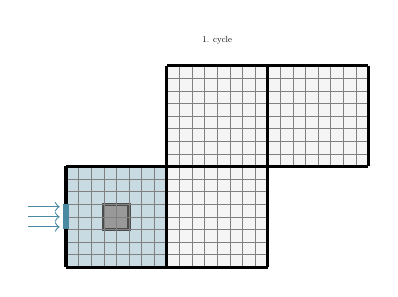
\begin{tikzpicture}
[
scale=0.32,
every node/.style ={scale=0.32},
Background/.style={rectangle,draw=black!04,fill=black!04, thin, minimum size = 4 cm},
BackgroundInflow/.style={rectangle,draw=black!04,fill={rgb,255:red,73;green,137;blue,162},opacity=0.3, thin, minimum size = 4 cm},
Obstruction/.style={rectangle,draw=black!70,fill=black!40, very thick, minimum size=1cm},
Finegrid/.style={step=0.5cm,gray,very thin},
Thickline/.style={-,draw=black!100,fill=black!02, very thick},
Thinline/.style={draw=black!100,fill=black!02, very thin},
Inflow/.style={-,draw={rgb,255:red,73;green,137;blue,162},line width=0.8mm},
Inarrow/.style={->,draw={rgb,255:red,73;green,137;blue,162},thin},
Outflow/.style={-,draw=blue!60,,line width=0.8mm},
Ball/.style={circle, draw=black!40, fill=red!20, thin, minimum size=3.5mm},
Circle/.style={circle,draw=black!40,fill=black!06,thin,minimum size=35.5mm},
Rectangle/.style={rectangle,draw=black!10,fill=white,inner xsep=0pt, inner ysep=0pt,},
Box/.style= {very thin, rectangle, inner xsep=10pt, inner ysep=10pt,},
ComArrow/.style={<->,semithick,draw=red!70},
]

\node[BackgroundInflow] at (2,2) {};
\node[Background] at (6,2) {};
\node[Background] at (6,6) {};
\node[Background] at (10,6) {};

\node[Obstruction] at (2,2) {};

\draw[Finegrid] (0,0) grid (8,4);
\draw[Finegrid] (4,4) grid (12,8);

\draw[Thickline] (0,0)--(8,0);
\draw[Thickline] (4,8)--(12,8);
\draw[Thickline] (0,4)--(4,4);
\draw[Thickline] (8,4)--(12,4);

\draw[Thickline] (0,0)--(0,4);
\draw[Thickline] (4,8)--(12,8);
\draw[Thickline] (4,4)--(4,8);
\draw[Thickline] (8,0)--(8,4);
\draw[Thickline] (12,4)--(12,8);

\draw[Thickline] (4,0)--(4,4);
\draw[Thickline] (4,4)--(8,4);
\draw[Thickline] (8,4)--(8,8);

\draw[Inflow]   (0,1.5)--(0,2.5);
\draw[Inarrow]  (-1.5,1.6)--(-0.25,1.6);
\draw[Inarrow]  (-1.5,2.0)--(-0.25,2.0);
\draw[Inarrow]  (-1.5,2.4)--(-0.25,2.4);
%\draw[Outflow]  (12,4)--(12,8);

%\draw[ComArrow](3.0,2)--(5.0,2);

\node [Box] (Box) at (6.0,9.0){{\HUGE 1. cycle}};

\end{tikzpicture}

\end{minipage}
\begin{minipage}{3.9cm}
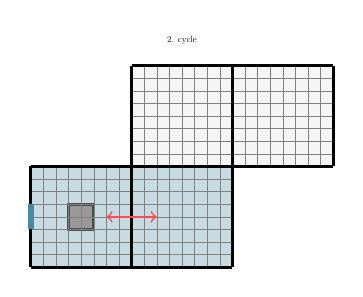
\begin{tikzpicture}
[
scale=0.32,
every node/.style ={scale=0.32},
Background/.style={rectangle,draw=black!04,fill=black!04, thin, minimum size = 4 cm},
BackgroundInflow/.style={rectangle,draw=black!04,fill={rgb,255:red,73;green,137;blue,162},opacity=0.3, thin, minimum size = 4 cm},
Obstruction/.style={rectangle,draw=black!70,fill=black!40, very thick, minimum size=1cm},
Finegrid/.style={step=0.5cm,gray,very thin},
Thickline/.style={-,draw=black!100,fill=black!02, very thick},
Thinline/.style={draw=black!100,fill=black!02, very thin},
Inflow/.style={-,draw={rgb,255:red,73;green,137;blue,162},line width=0.8mm},
Inarrow/.style={->,draw={rgb,255:red,73;green,137;blue,162},thin},
Outflow/.style={-,draw=blue!60,,line width=0.8mm},
Ball/.style={circle, draw=black!40, fill=red!20, thin, minimum size=3.5mm},
Circle/.style={circle,draw=black!40,fill=black!06,thin,minimum size=35.5mm},
Rectangle/.style={rectangle,draw=black!10,fill=white,inner xsep=0pt, inner ysep=0pt,},
Box/.style= {very thin, rectangle, inner xsep=10pt, inner ysep=10pt,},
ComArrow/.style={<->,semithick,draw=red!70},
]

\node[BackgroundInflow] at (2,2) {};
\node[BackgroundInflow] at (6,2) {};
\node[Background] at (6,6) {};
\node[Background] at (10,6) {};

\node[Obstruction] at (2,2) {};

\draw[Finegrid] (0,0) grid (8,4);
\draw[Finegrid] (4,4) grid (12,8);

\draw[Thickline] (0,0)--(8,0);
\draw[Thickline] (4,8)--(12,8);
\draw[Thickline] (0,4)--(4,4);
\draw[Thickline] (8,4)--(12,4);

\draw[Thickline] (0,0)--(0,4);
\draw[Thickline] (4,8)--(12,8);
\draw[Thickline] (4,4)--(4,8);
\draw[Thickline] (8,0)--(8,4);
\draw[Thickline] (12,4)--(12,8);

\draw[Thickline] (4,0)--(4,4);
\draw[Thickline] (4,4)--(8,4);
\draw[Thickline] (8,4)--(8,8);

\draw[Inflow]   (0,1.5)--(0,2.5);
%\draw[Inarrow]  (-1,1.6)--(-0.25,1.6);
%\draw[Inarrow]  (-1,2.0)--(-0.25,2.0);
%\draw[Inarrow]  (-1,2.4)--(-0.25,2.4);
%\draw[Outflow]  (12,4)--(12,8);

\draw[ComArrow](3.0,2)--(5.0,2);

\node [Box] (Box) at (6.0,9.0){{\HUGE 2. cycle}};

\end{tikzpicture}

\end{minipage}
\begin{minipage}{3.9cm}
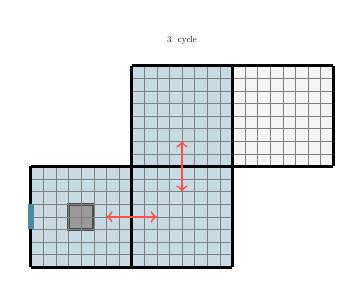
\begin{tikzpicture}
[
scale=0.32,
every node/.style ={scale=0.32},
Background/.style={rectangle,draw=black!04,fill=black!04, thin, minimum size = 4 cm},
BackgroundInflow/.style={rectangle,draw=black!04,fill={rgb,255:red,73;green,137;blue,162},opacity=0.3, thin, minimum size = 4 cm},
Obstruction/.style={rectangle,draw=black!70,fill=black!40, very thick, minimum size=1cm},
Finegrid/.style={step=0.5cm,gray,very thin},
Thickline/.style={-,draw=black!100,fill=black!02, very thick},
Thinline/.style={draw=black!100,fill=black!02, very thin},
Inflow/.style={-,draw={rgb,255:red,73;green,137;blue,162},line width=0.8mm},
Inarrow/.style={->,draw={rgb,255:red,73;green,137;blue,162},thin},
Outflow/.style={-,draw=blue!60,,line width=0.8mm},
Ball/.style={circle, draw=black!40, fill=red!20, thin, minimum size=3.5mm},
Circle/.style={circle,draw=black!40,fill=black!06,thin,minimum size=35.5mm},
Rectangle/.style={rectangle,draw=black!10,fill=white,inner xsep=0pt, inner ysep=0pt,},
Box/.style = {very thin, rectangle, inner xsep=10pt, inner ysep=10pt,},
ComArrow/.style= {<->,semithick,draw=red!70},
]

\node[BackgroundInflow] at (2,2) {};
\node[BackgroundInflow] at (6,2) {};
\node[BackgroundInflow] at (6,6) {};
\node[Background] at (10,6) {};

\node[Obstruction] at (2,2) {};

\draw[Finegrid] (0,0) grid (8,4);
\draw[Finegrid] (4,4) grid (12,8);

\draw[Thickline] (0,0)--(8,0);
\draw[Thickline] (4,8)--(12,8);
\draw[Thickline] (0,4)--(4,4);
\draw[Thickline] (8,4)--(12,4);

\draw[Thickline] (0,0)--(0,4);
\draw[Thickline] (4,8)--(12,8);
\draw[Thickline] (4,4)--(4,8);
\draw[Thickline] (8,0)--(8,4);
\draw[Thickline] (12,4)--(12,8);

\draw[Thickline] (4,0)--(4,4);
\draw[Thickline] (4,4)--(8,4);
\draw[Thickline] (8,4)--(8,8);

\draw[Inflow]   (0,1.5)--(0,2.5);
%\draw[Inarrow]  (-1,1.6)--(-0.25,1.6);
%\draw[Inarrow]  (-1,2.0)--(-0.25,2.0);
%\draw[Inarrow]  (-1,2.4)--(-0.25,2.4);
%\draw[Outflow]  (12,4)--(12,8);

\draw[ComArrow](3.0,2)--(5.0,2);
\draw[ComArrow](6,3.0)--(6,5.0);

\node [Box] (Box) at (6.0,9.0){{\HUGE 3. cycle}};


\end{tikzpicture}

\end{minipage}
\begin{minipage}{3.9cm}
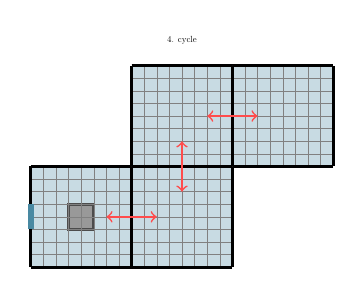
\begin{tikzpicture}
[
scale=0.32,
every node/.style ={scale=0.32},
Background/.style={rectangle,draw=black!04,fill=black!04, thin, minimum size = 4 cm},
BackgroundInflow/.style={rectangle,draw=black!04,fill={rgb,255:red,73;green,137;blue,162},opacity=0.3, thin, minimum size = 4 cm},
Obstruction/.style={rectangle,draw=black!70,fill=black!40, very thick, minimum size=1cm},
Finegrid/.style={step=0.5cm,gray,very thin},
Thickline/.style={-,draw=black!100,fill=black!02, very thick},
Thinline/.style={draw=black!100,fill=black!02, very thin},
Inflow/.style={-,draw={rgb,255:red,73;green,137;blue,162},line width=0.8mm},
Inarrow/.style={->,draw={rgb,255:red,73;green,137;blue,162},thin},
Outflow/.style={-,draw=blue!60,,line width=0.8mm},
Ball/.style={circle, draw=black!40, fill=red!20, thin, minimum size=3.5mm},
Circle/.style={circle,draw=black!40,fill=black!06,thin,minimum size=35.5mm},
Rectangle/.style={rectangle,draw=black!10,fill=white,inner xsep=0pt, inner ysep=0pt,},
Box/.style= {very thin, rectangle, inner xsep=10pt, inner ysep=10pt,},
ComArrow/.style= {<->,semithick,draw=red!70},
]

\node[BackgroundInflow] at (2,2) {};
\node[BackgroundInflow] at (6,2) {};
\node[BackgroundInflow] at (6,6) {};
\node[BackgroundInflow] at (10,6) {};

\node[Obstruction] at (2,2) {};

\draw[Finegrid] (0,0) grid (8,4);
\draw[Finegrid] (4,4) grid (12,8);

\draw[Thickline] (0,0)--(8,0);
\draw[Thickline] (4,8)--(12,8);
\draw[Thickline] (0,4)--(4,4);
\draw[Thickline] (8,4)--(12,4);

\draw[Thickline] (0,0)--(0,4);
\draw[Thickline] (4,8)--(12,8);
\draw[Thickline] (4,4)--(4,8);
\draw[Thickline] (8,0)--(8,4);
\draw[Thickline] (12,4)--(12,8);

\draw[Thickline] (4,0)--(4,4);
\draw[Thickline] (4,4)--(8,4);
\draw[Thickline] (8,4)--(8,8);

\draw[Inflow]   (0,1.5)--(0,2.5);
%\draw[Inarrow]  (-1,1.6)--(-0.25,1.6);
%\draw[Inarrow]  (-1,2.0)--(-0.25,2.0);
%\draw[Inarrow]  (-1,2.4)--(-0.25,2.4);
%\draw[Outflow]  (12,4)--(12,8);

\draw[ComArrow](3.0,2)--(5.0,2);
\draw[ComArrow](6,3.0)--(6,5.0);
\draw[ComArrow](7.0,6)--(9.0,6);

\node [Box] (Box) at (6.0,9.0){{\HUGE 4. cycle}};

\end{tikzpicture}

\end{minipage}
\caption[Delayed information transfer of the mesh-wise FFT solver]{Delayed information transfer of the mesh-wise FFT solver for the 2D pipe geometry: New information can only be passed across the whole domain by successively using the next-neighbor communications between adjacent meshes.}
\label{FIG_SCARC_mesh_wise_transfer}
\end{figure}
\end{center}



There is yet another important issue regarding the treatment of internal obstructions that should be considered:
Since the use of the FFT-solver is basically limited to structured meshes, it is not possible to specify internal boundary conditions and the velocity field may penetrate into internal solids as already explained in Section (\ref{SEC_SCARC_poisson}). 
%
In order to compensate this undesired effect an additional iterative correction strategy based on a {\it Direct Forcing Immersed Boundary Method}~\cite{Fadlun:2000} is used in FDS: In every time step the mesh-wise FFT algorithm is not applied only once but multiple times until a specified {\it velocity tolerance} for the remaining velocity error along internal obstructions has been reached. This iterative corrective process will be denoted as {\it pressure iteration} below.

Furthermore, although the pressure term $\cH$ is continuous at mesh interfaces, the finite-difference of its gradient is not such that the normal components of velocity also may be different at common mesh interfaces. Thus, the above pressure iteration is also used to drive the velocity normals to match up to the specified velocity tolerance along common mesh interfaces.

For both, the internal obstructions and the mesh interfaces, the required velocity tolerance and the maximum allowed number of correction iterations can be specified by the quantities {\ct VELOCITY\_TOLERANCE} and {\ct  MAX\_PRESSURE\_ITERATIONS} 
in the {\ct \&PRES}-namelist. By default, a velocity tolerance of ''characteristic mesh size'' divided by 10 and a maximum of 10 iterations is used. Fig.~\ref{FIG_SCARC_multi_pipe_fft_presite} illustrates this procedure graphically.
More detailed information about the underlying procedure can be obtained in the FDS Technical Reference Guide~\cite{McGrattan:2018:TG}.

\begin{figure}[ht]
\begin{center}
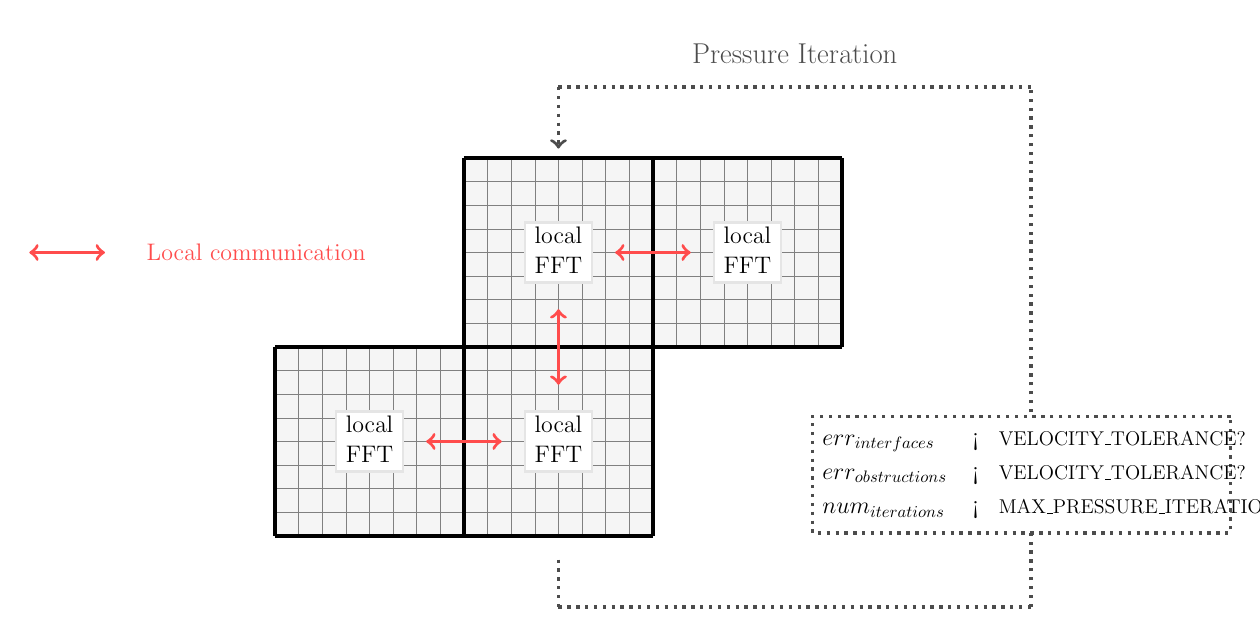
\begin{tikzpicture}
[
scale=0.6,
every node/.style={scale=0.6},
Background/.style={rectangle,draw=black!04,fill=black!04, thin, minimum size = 4 cm},
Obstruction/.style={rectangle,draw=black!70,fill=black!40, very thick, minimum size=1cm},
Finegrid/.style={step=0.5cm,gray,very thin},
Thickline/.style={-,draw=black!100,fill=black!02, very thick},
Thinline/.style={draw=black!100,fill=black!02, very thin},
Ball/.style={circle, draw=black!40, fill=red!20, thin, minimum size=3.5mm},
Circle/.style={circle,draw=black!40,fill=black!06,thin,minimum size=35.5mm},
Rectangle/.style={rectangle,draw=black!10,fill=white,inner xsep=0pt, inner ysep=0pt,},
Box/.style= {very thin, rectangle, inner xsep=10pt, inner ysep=10pt,},
DotBox/.style= {very thick, rectangle, inner xsep=0pt, inner ysep=8pt, dotted, fill=white, draw=black!70,},
ComArrow/.style= {<->,very thick, draw=red!70,},
DotArrow/.style= {<-, thick, dotted, draw=black!70,},
DotLine/.style= {very thick, dotted, draw=black!70,},
]

\node[Background] at (  2,2) {};
\node[Background] at (  6,2) {};
\node[Background] at (  6,6) {};
\node[Background] at (10,6) {};

\node[Obstruction] at (2,2) {};

\draw[Finegrid] (0,0) grid (  8,4);
\draw[Finegrid] (4,4) grid (12,8);

\draw[Thickline] (0,0)--(  8,0);
\draw[Thickline] (4,8)--(12,8);
\draw[Thickline] (0,4)--(  4,4);
\draw[Thickline] (8,4)--(12,4);

\draw[Thickline] (  0,0)--(  0,4);
\draw[Thickline] (  4,8)--(12,8);
\draw[Thickline] (  4,4)--(  4,8);
\draw[Thickline] (  8,0)--(  8,4);
\draw[Thickline] (12,4)--(12,8);

\draw[Thickline] (4,0)--(4,4);
\draw[Thickline] (4,4)--(8,4);
\draw[Thickline] (8,4)--(8,8);

\node[Rectangle] at (  2,2.0) {\Large \begin{tabular}{c} local \\ FFT\end{tabular}};
\node[Rectangle] at (  6,2.0) {\Large \begin{tabular}{c} local \\ FFT\end{tabular}};
\node[Rectangle] at (  6,6.0) {\Large \begin{tabular}{c} local \\ FFT\end{tabular}};
\node[Rectangle] at (10,6.0) {\Large \begin{tabular}{c} local \\ FFT\end{tabular}};

\draw[ComArrow](3.2,2)--(4.8,2);
\draw[ComArrow](6,3.2)--(6,4.8);
\draw[ComArrow](7.2,6)--(8.8,6);

\draw[ComArrow](-5.2,6)--(-3.6,6);
\node [Box,red!70] (box) at (-0.4,6){%
    \begin{minipage}{0.56\textwidth}
    \begin{center}
        {\Large Local communication}
    \end{center}
    \end{minipage}};

\draw[  -,DotLine](6,-0.5)--(6,-1.5);
\draw[  -,DotLine](6,-1.5)--(16,-1.5);
\draw[  -,DotLine](16,-1.5)--(16,9.5);
\draw[  -,DotLine](6,9.5)--(16,9.5);
\draw[->,DotLine](6,9.5)--(6,8.2);

\node [DotBox] (box) at (15.8,1.3){%
    \begin{minipage}{0.73\textwidth}    
    \begin{center}
    \begin{tabular}{lclc|c|}
       {\ct  \Large $err_{interfaces}$} & {\Large <} & {\ct \large VELOCITY\_TOLERANCE?}            \\[2ex]
       {\ct  \Large $err_{obstructions}$} & {\Large <} & {\ct \large VELOCITY\_TOLERANCE?}         \\[2ex]
       {\ct  \Large $num_{iterations}$ }    &{\Large <} & {\ct \large MAX\_PRESSURE\_ITERATIONS?} \\
    \end{tabular}
    \end{center}
    \end{minipage}};

\node [Box, black!70] (box) at (11,10.2){\LARGE Pressure Iteration};

\end{tikzpicture}

\caption[Mesh-wise FFT-methods with pressure correction]{Repeated use of the FFT pressure solver for a 2D pipe geometry: In the scope of a surrounding pressure iteration the mesh-wise FFT's are performed multiple times until the error related to the normal components of velocity along internal obstructions and mesh interfaces has been driven below a specified velocity tolerance.}
\label{FIG_SCARC_multi_pipe_fft_presite}
\end{center}
\end{figure}

Certainly, the increased number of mesh-wise FFT solutions leads to a higher computational effort. Nevertheless, for a multitude of cases, especially for relatively small mesh numbers or in steady-state like situations, only less corrective iterations are needed and convergence is achieved very quickly.
Increasing the number of subdomains may worsen the convergence and accuracy behaviour associated with a noticeable increase of computational costs.
%, possibly up to divergence at a (problem-dependent) critical number of subdomains. 

Especially, for extended geometries with a big number of meshes (i.e.\ tunnels) and/or transient boundary conditions this purely local strategy may experience difficulties to reproduce the rapid propagation of information for elliptic problems fast enough and convergence of the pressure iteration may be slow.
In particular, these situations make the development of alternative solution concepts appear necessary and have driven their development forward.

% ----------------------------------------------------------------------------------------------------------------------------------------
% LU solver
% ----------------------------------------------------------------------------------------------------------------------------------------
\subsection{Parallel $\boldmath{LU}$-factorization}
\label{SEC_SCARC_lu_decomposition}
Within the framework of the Gaussian elimination algorithm, many direct algorithms rely on the 'lower-upper'-factorization of the system matrix, $LU = PAQ$, 
with suitable permutation matrices $P$ and $Q$ and the triangular matrices $L$ and $U$, see Fig.~\ref{FIG_SCARC_lu_decomposition}. 
The solution of Equation (\ref{EQ_SCARC_single_system}) can then be obtained using a forward substitution step, $Ly=P^Tb$, followed by a backward substitution step, $U(Q^Tx)=y$.
If $A$ is symmetric, a {\it Cholesky factorization} $PAP^T=LL^T$ can be applied.

The whole process can be subdivided into three phases: 
(i) a {\it reordering phase}  where the matrix is analyzed to produce an ordering which allows a more efficient factorization,
(ii) a {\it factorization phase} where the $LU$-factorization is actually computed and stored, 
(iii) a {\it solution phase} where the forward and backward substitution is performed.
Typically, the factorization phase (ii) requires the most computing time while the solution phase (iii) is an order of magnitude faster.

\begin{figure}[ht]
\begin{center}
\begin{tikzpicture}
[ 
  every node/.style ={scale=0.5},
 ]
\tikzstyle{every path}=[draw, line width=0.3mm];
\def\bracket{
  \draw[-] (1,10) -| (0,0) -- (1,0);
  \draw[-] (9,10) -| (10,0) -- (9,0);
}
\def\basecoords{ 
    \coordinate (-v1) at (1,1);
    \coordinate (-v2) at (9,1);
    \coordinate (-v3) at (9,9);
    \coordinate (-v4) at (1,9);
}
\tikzset{pics/.cd,
  my square/.style={code={\basecoords\fill [#1] (-v1) rectangle (-v3);\bracket}},
  my trileft/.style={code={\basecoords\fill [#1] (-v2) -- (-v4) -- (-v1);\bracket}},
  my triright/.style={code={\basecoords\fill [#1] (-v2) -- (-v3) -- (-v4);\bracket}}
 }

\pic[local bounding box=A,scale=0.4]  at (0,0)                              {my square={opacity=0.3,gray} };
\pic[local bounding box=B,scale=0.4,right=2 cm of A.south east] {my trileft   ={opacity=0.3,gray}};
\pic[local bounding box=C,scale=0.4,right=2 cm of B.south east] {my triright ={opacity=0.3,gray}};

\node[scale=2] (a) at ($(A.east)!0.5!(B.west)$) {$=$};
\node[scale=2] (b) at ($(B.east)!0.5!(C.west)$) {$\times$};

\node[scale=2] (At) at ([shift={(80:0.5)}]$(A.north)$) {$A$};
\node[scale=2] (Bt) at ([shift={(80:0.5)}]$(B.north)$) {$L$};
\node[scale=2] (Ct) at ([shift={(80:0.5)}]$(C.north)$) {$U$};
\end{tikzpicture}

\end{center}
\caption{Decomposition of $A$ into a lower triangular matrix $L$ and an upper triangular matrix $U$}
\label{FIG_SCARC_lu_decomposition}
\end{figure}


While $LU$-decomposition was originally developed for serial applications, there are optimized parallel variants today which calculate a distributed LU decomposition based on a global discretization with corresponding global Poisson matrix. In FDS a solver named \uglmat{} is used, which is built on the optimized parallel {\ct Cluster\_Sparse\_Solver} of the Intel\textsuperscript{\textregistered} MKL library.

Due to its domain-spanning character the factorization phase (ii) is very communication-intensive which is reflected in long calculation times for initialization.
However, as long as there are no geometric changes in the computational domain during the simulation (e.g. by the ``opening'' or ``closing'' of obstructions), this only has to be done once.
In every FDS time iteration the solution of the respective Poisson equation is simply based on a forward and backward substitution step on every single mesh with respect to the stored factorization which can be done much faster.

\newpage
Figure \ref{FIG_SCARC_uglmat} illustrates the $LU$-decomposition for the 2D-pipe example. The dashed lines between the single meshes indicate that the whole method is based on the global Poisson matrix and the mutually required entries are communicated between the single meshes.

\begin{figure}[ht]
\centering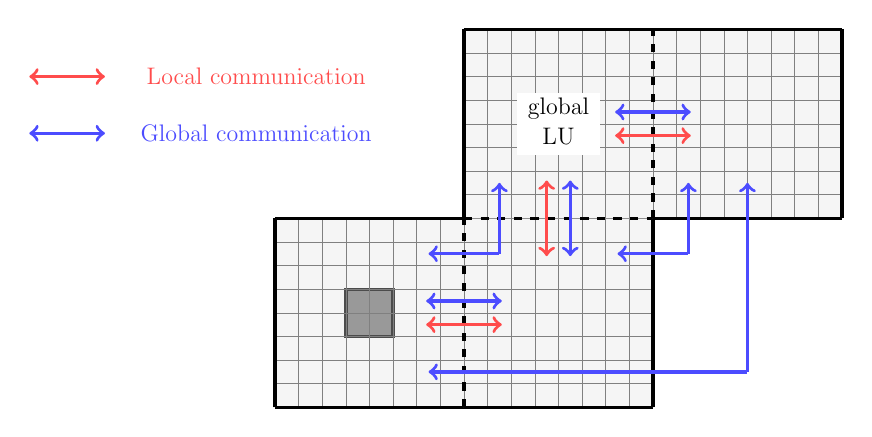
\begin{tikzpicture}
[
scale=0.6,
every node/.style={scale=0.6},
Background/.style={rectangle,draw=black!04,fill=black!04, thin, minimum size = 4 cm},
Obstruction/.style={rectangle,draw=black!70,fill=black!40, very thick, minimum size=1cm},
GlobalBorder/.style={-.,draw=black!100,  thin},
Finegrid/.style={step=0.5cm,gray,very thin},
Thickline/.style={-,draw=black!100,fill=black!02, very thick},
ThickDashedline/.style={-,draw=black!100,fill=black!02, very thick, dashed},
Thinline/.style={draw=black!100,fill=black!02, very thin},
Ball/.style={circle, draw=black!40, fill=red!20, thin, minimum size=3.5mm},
Circle/.style={circle,draw=black!40,fill=black!06,thin,minimum size=35.5mm},
Rectangle/.style={rectangle,draw=black!0,fill=white,inner xsep=0pt, inner ysep=0pt,},
Box/.style= {very thin, rectangle, inner xsep=10pt, inner ysep=10pt,},
DotBox/.style= {very thick, rectangle, inner xsep=10pt, inner ysep=10pt, dotted, fill=white, draw=black!70,},
ComRedArrow/.style= {very thick, draw=red!70,},
ComBlueArrow/.style= {very thick, draw=blue!70,},
DotArrow/.style= {<-, thick, dotted, draw=black!70,},
DotLine/.style= {very thick, dotted, draw=black!70,},
]

%\draw[GlobalBorder, fill=black!10] (-1.2,-1.2)--(13.2,-1.2)--(13.2,9.2)--(-1.2,9.2)--(-1.2,-1.2);

\node[Background] at (  2,2) {};
\node[Background] at (  6,2) {};
\node[Background] at (  6,6) {};
\node[Background] at (10,6) {};

\node[Obstruction] at (2,2) {};

\draw[Finegrid] (0,0) grid (  8,4);
\draw[Finegrid] (4,4) grid (12,8);

\draw[Thickline] (0,0)--(  8,0);
\draw[Thickline] (4,8)--(12,8);
\draw[Thickline] (0,4)--(  4,4);
\draw[Thickline] (8,4)--(12,4);

\draw[Thickline] (  0,0)--(  0,4);
\draw[Thickline] (  4,8)--(12,8);
\draw[Thickline] (  4,4)--(  4,8);
\draw[Thickline] (  8,0)--(  8,4);
\draw[Thickline] (12,4)--(12,8);

\draw[ThickDashedline] (4,0)--(4,4);
\draw[ThickDashedline] (4,4)--(8,4);
\draw[ThickDashedline] (8,4)--(8,8);

\node[Rectangle] at (  6,6.0) {\Large \begin{tabular}{c} global \\ LU\end{tabular}};

\draw[<->,ComRedArrow](3.2,1.75)--(4.8,1.75);
\draw[<->,ComRedArrow](5.75,3.2)--(5.75,4.8);
\draw[<->,ComRedArrow](7.2,5.75)--(8.8,5.75);

\draw[<->,ComBlueArrow](3.2,2.25)--(4.8,2.25);
\draw[<->,ComBlueArrow](6.25,3.2)--(6.25,4.8);
\draw[<->,ComBlueArrow](7.2,6.25)--(8.8,6.25);

\draw[<-, ComBlueArrow](3.25,3.25)--(4.75,3.25);
\draw[->, ComBlueArrow](4.75,3.25)--(4.75,4.75);
\draw[<-, ComBlueArrow](7.25,3.25)--(8.75,3.25);
\draw[->, ComBlueArrow](8.75,3.25)--(8.75,4.75);
\draw[<-, ComBlueArrow](3.25,0.75)--(10,0.75);
\draw[->, ComBlueArrow](10.0,0.75)--(10,4.75);

\draw[<->,ComRedArrow](-5.2,7.0)--(-3.6,7.0);
\node [Box,red!70] (box) at (-0.4,7.0){%
    \begin{minipage}{0.56\textwidth}
    \begin{center}
        {\Large Local communication}
    \end{center}
    \end{minipage}};
    
\draw[<->,ComBlueArrow](-5.2,5.8)--(-3.6,5.8);
\node [Box,blue!70] (box) at (-0.4,5.8){%
    \begin{minipage}{0.56\textwidth}
    \begin{center}
        {\Large Global communication}
    \end{center}
    \end{minipage}};

\end{tikzpicture}

\caption{Decomposition of $A$ into a lower triangular matrix $L$ and an upper triangular matrix $U$}
\label{FIG_SCARC_uglmat}
\end{figure}

A main disadvantage of this approach is that less benefit can be drawn from a very convenient property of 
the Poisson matrix $A$, namely its intrinsic {\it sparsity}:
Even though $A$ has only very few non-zero entries compared to the total number of possible entries $n^2$, 
%which are grouped in single diagonal bands (7 bands in case of the 7-point stencil), 
the $LU$-factorization process leads to {\it fill-in}, i.e.\ it produces non-zero entries in $L$ and $U$ where $A$ was zero before.
This relation is illustrated in Fig.~\ref{FIG_SCARC_lu_memory_spy}.
For a simple 3D-cube geometry which is refined into $16^3$ cells it shows the sparsity pattern of the Poisson matrix $A$
and the lower triangular matrix $L$ of its $LU$-decomposition.

\begin{figure}[ht]
\begin{center}
\includegraphics[width=0.4\textwidth]{\figPath/spy_A.png}\qquad\qquad\qquad
\includegraphics[width=0.4\textwidth]{\figPath/spy_L.png}\\
\end{center}
\caption[Sparsity patterns in case of a $LU$-decomposition for a refined 3D-cube with $16^3$ cells]{
Sparsity patterns in case of the $LU$-decomposition for a refined 3D-cube with $16^3$ cells.
(Left) Poisson matrix $A$ with about 27 thousand non-zeros; (Right) Lower triangular matrix $L$ with nearly 1 million non-zeros;
}
\label{FIG_SCARC_lu_memory_spy}
\end{figure}

\newpage
The computing and storing of both triangular matrices can become prohibitively expensive, especially in case of huge systems of equations with many  millions of unknowns. This is true even if only the lower triangular matrix has to be stored for symmetric problems.

The example of the 3D-cube is taken up again in order to show the magnitudes of memory requirements to be expected here.
In case that the cube is refined from $16^3$ up to $128^3$ cells, Fig.~\ref{FIG_SCARC_lu_memory_need} compares
the number of non-zero entries of $L$ with those of $A$. Apparently the ratio dramatically deteriorates as the grid is refined. 
For the finest grid resolution of $128^3$ cells the matrix $L$ has about 2.18 billions %2,178,331,820 
of non-zeros whereas $A$ only has about 8.34 millions of non-zeros, %8,339,456 
corresponding to a ratio of about 238. Note, that for $A$ only its lower triangular and diagonal part must be stored due to its symmetry.

\begin{figure}[ht]
\centering\includegraphics[width=0.6\textwidth]{\figPath/lu_memory_needs.png}\\[2ex]
\caption[Memory needs for the $LU$-decomposition]{
Number of non-zero entries in the Poisson matrix $A$ (green) and the lower triangular matrix $L$ (blue) of its $LU$-decomposition for different refinements of a 3D-cube from $16^3$ up to $128^3$ cells. The resulting ratio of $L$ to  $A$ is indicated at top of the blue bars. 
}
\label{FIG_SCARC_lu_memory_need}
\end{figure}

For realistically large CFD-problems the resulting additional storage requirements can  exceed the capacity of the available computing system in the worst case.
Thus, when considering the computational efficiency of $LU$-methods for a given application the resulting fill-in is a decisive criterion. 


